Traditionally, events in neutrino experiments based on the LArTPC technology are reconstructed using a set of algorithms that are tuned independently and rely on hand-engineered features. In recent years, machine learning (ML) has become a powerful tool in computer science, consistently breaking performance records in computer vision and natural language processing. The highly-visual nature of LArTPC data makes it a natural candidate for machine learning applications: the images of particles are easy to interpret by eye, but it is often hard to programmatically design algorithms to extract high-level features suitable for physics analyses. Moreover, the physics goals of the SBN Program assume high-purity and high-efficiency automatic selections that have so far remained out of reach of traditional pattern recognition techniques. This chapter describes the event reconstruction based on neural networks employed in the ICARUS experiment. Section \ref{sec:neural_networks} provides an overview of the different types of neural networks used in the ICARUS ML event reconstruction. An overview of the generators used to produce the training sample is provided in Section \ref{sec:training_datasets}. Section \ref{sec:ml_full_chain} describes the full ML chain used in the ICARUS ML event reconstruction, from the input data to the final output. Finally, Section \ref{sec:post_processing} describes the post-processing steps that are applied to the output of the neural networks to extract the final physics quantities.

\subsection{Neural Networks}
\label{sec:neural_networks}

Artificial neural networks can be described as a family of parameterized functional approximations that are inspired by the structure and function of the biological neural networks in the brain. The basic building block of a neural network is the artificial neuron, which is a simple computational unit that receives a signal from connected neurons and produces an output signal. The output signal is computed by some non-linear function of the weighted sum of the input signals. Typically, neurons are aggregated into layers and the layers are stacked to form a network. Signals travel from the input layer to the output layer, possibly traversing multiple intermediate ``hidden'' layers, with the output of one layer serving as the input to the next layer. A neural network is said to be ``deep'' if it has more than one hidden layer. Figure \ref{fig:neural_network} shows a schematic representation of a simple neural network with one hidden layer.

\begin{figure}
    \centering
    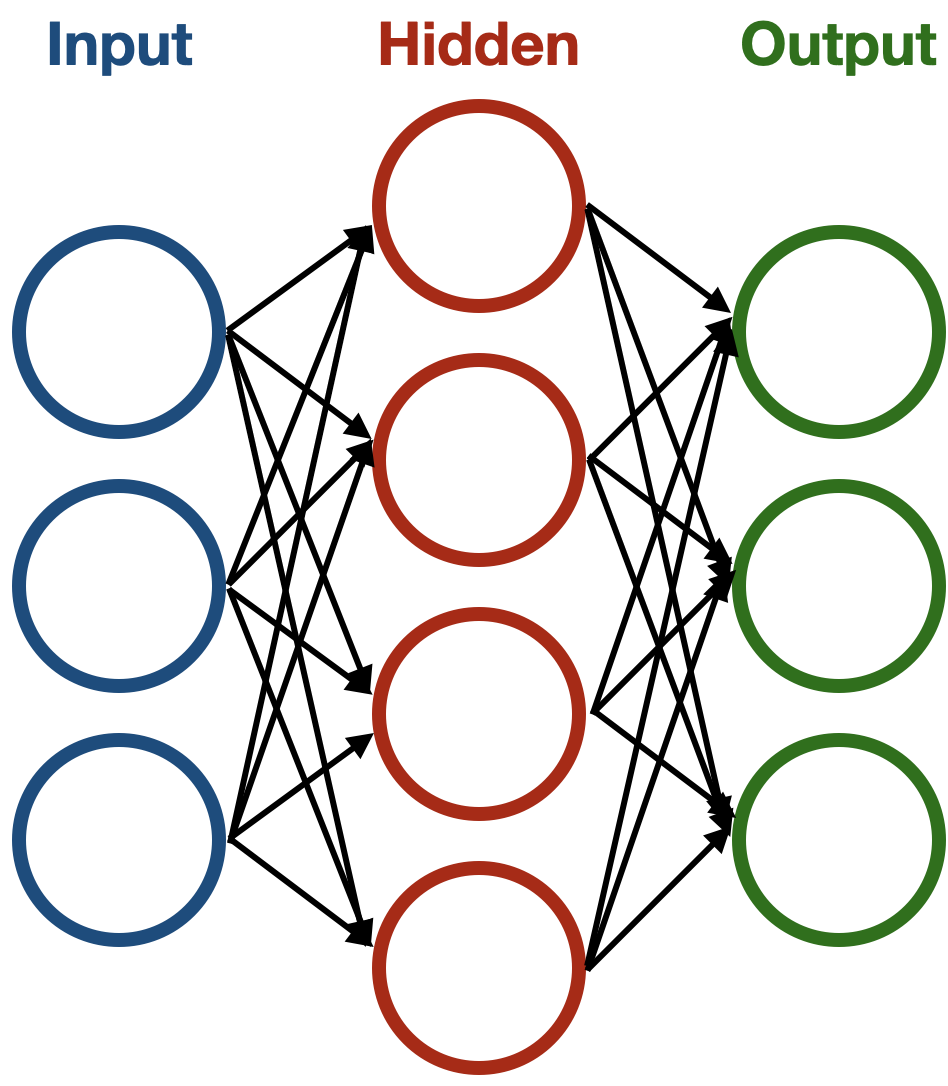
\includegraphics[width=0.5\textwidth]{figures/mlreco/neural_network.png}
    \caption{Schematic representation of a simple neural network with one hidden layer.}
    \label{fig:neural_network}
\end{figure}

The parameters of a neural network are typically optimized through gradient-based methods that serve to minimize a loss function. The loss function is a measure of the difference between the predicted output of the network and the target value. In a supervised learning setting, the target value is known and the network is trained to predict this value. This necessitates the use of labeled data, where the target value/category is known. For applications in neutrino physics, the role of a training sample is played by simulated data, where the truth information is known from the simulation. The trained network can then be applied to real data, where the target value is not known, to make predictions. 

\subsubsection{Convolutional Neural Networks}
\label{sec:cnn}

The convolutional neural network (CNN) is a type of neural network that is particularly well-suited for image recognition tasks. Compared to basic neural networks, CNNs make the additional assumption that most of the relevant information exists in a local neighborhood around the signal of interest. This is a natural description of LArTPC data, where the images of particles are highly structured and the local features are important for classification of particles/events. This requirement of sensitivity to local features motivates the use of convolutional layers in CNNs. A convolutional layer computes the dot product between its weights and a small region of the input data. The spatial extent of this region is called the receptive field of the neuron. This convolutional operation is iteratively moved across the entire input image producing an activation map, which may be stacked with other activation maps to obtain the output. Pooling layers are often used in conjunction with convolutional layers to reduce the spatial dimensions of the input data. This is done by aggregating the values of neighboring pixels in the input data with an operation such as max pooling or average pooling. A pooling layer also has the effect of expanding the receptive field as the aggregation method pulls in information from a larger region of the input data.

The restricted spatial extent of the convolutional layers allows CNNs to have fewer parameters than fully-connected networks, which would be computationally prohibitive for images of the size of LArTPC data. The use of shared weights in the convolutional layers also allows CNNs to learn translation-invariant features; that is, features that are detected regardless of their position in the image. This is particular desirable for LArTPC data where the position of the particle and the underlying space points in the detector is not relevant for the classification task.

\subsubsection{Graph Neural Networks}
\label{sec:gnn}

Graph neural networks (GNN) are a class of neural networks that are well-suited for datasets with a natural relational structure. The input data in a GNN is represented as a set of nodes and edges, where the nodes represent the entities of interest and the edges represent the relationships between the entities. The key design principle in GNNs is the use of message passing, a process by which the features of each node and edge are updated by aggregating the features of its neighbors. This is an iterative process performed across the entire graph, thus allowing the network to learn complex relationships between the nodes. Among all graph learning tasks, two are of particular relevance in this analysis:

\begin{itemize}
    \item \textbf{Node-learning tasks}: tasks that involve predicting the classification of a node. In the context of LArTPC data, an example is the classification of a particle as a muon or a primary particle coming out of the interaction vertex.
    \item \textbf{Edge-learning tasks}: tasks that involve predicting the classification of an edge. To relate to LArTPC data, an example is the classification of two particles being part of the same interaction, or of two shower fragments belonging to the same parent shower. 
\end{itemize}

\subsection{Training Datasets}
\label{sec:training_datasets}

The training of neural networks requires a labeled dataset, where the true output is known. In the context of LArTPC data, the labeled dataset is provided by the simulation of the detector response to a set of known particles. In order to avoid potential biases due to assumptions of particular physics models governing cosmic ray and neutrino generation, the reconstruction chain is trained using a set of simulated events produced by two physics-agnostic generators:

\begin{itemize}
    \item \textbf{Multi-Particle Vertex (MPV)}: this generator produces a set of up to $N$ particles originating from a common vertex. These particles include electrons, positrons, photons, muons, anti-muons, both negatively-charged and positively-charged pions, and protons.
    \item \textbf{Multi-Particle Rain (MPR)}: this generator produces a set of up to $M$ isolated particles. These particles include electrons, positrons, muons, anti-muons, and protons.
\end{itemize}

\noindent
The MPV generator is meant to emulate a pseudo-neutrino interaction with multiple particles emitted from a common vertex, whereas the MPR generator produces interactions that are similar to those produced by cosmic rays. For each particle, the generators are configured with a range of kinetic energies than can be assigned as well as a maximum particle multiplicity. The kinetic energy is drawn from a uniform distribution within the configurable range. The maximum particle multiplicity for a given vertex is enforced by only drawing particles of types that are not already at their preconfigured maximum.

The range of all parameters controlling the generation of training events is ideally a superset of the phase space observed in ICARUS data and Monte Carlo simulation. This is to avoid regions of phase space where performance of the reconstruction is worse due to relatively few encounters of events in this region of phase space in the training sample. For example, the reconstruction may struggle to correctly identify low-energy protons if the training sample does not have sufficiently high representation of low-energy protons. The particles generated by these generators are fed into the full detector simulation. This allows for the network to be trained on events that represent detector effects to the extent that they are modeled in the simulation.

\subsection{The ICARUS Machine Learning Analysis Chain}
\label{sec:ml_full_chain}

The Neutrino ML group at SLAC has developed an end-to-end, ML-based reconstruction chain for the ICARUS experiment. The chain consists of a hierarchical set of neural networks that are optimizable end-to-end. The two types of neural networks described in the preceding section are employed: CNNs and GNNs. The full chain is shown schematically in Figure \ref{fig:mlreco_schematic} and each stage is summarized in Table \ref{fig:mlreco_nn}. This section reviews each stage of the chain in order, starting from the voxel-level tasks and building up to the high-level particle- and interaction-level classifications. 

\begin{figure}
    \centering
    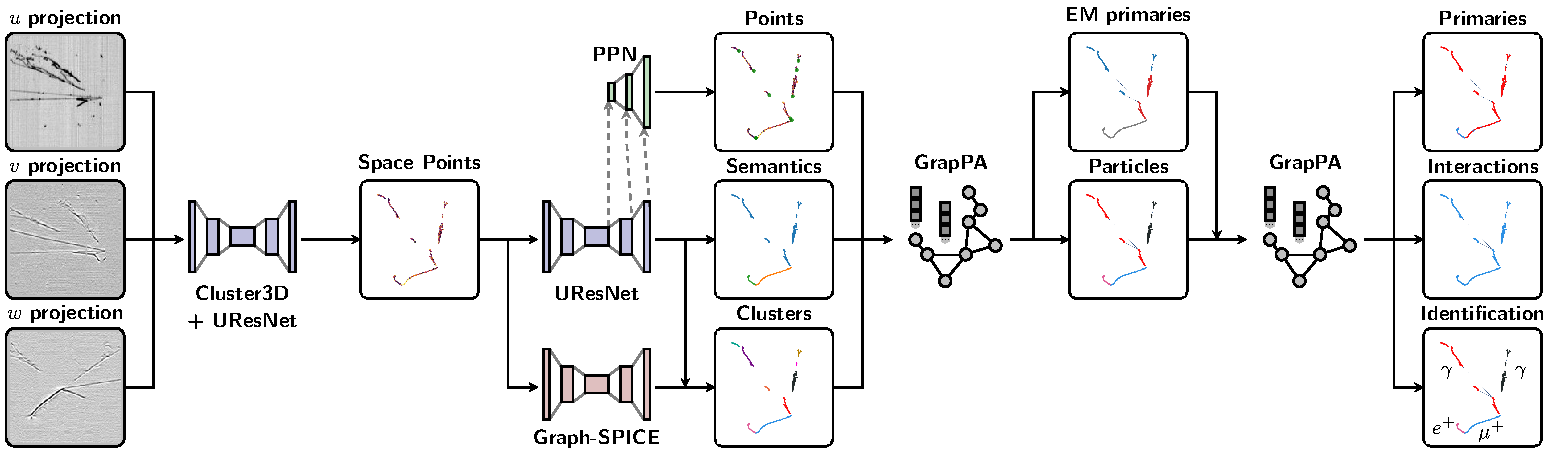
\includegraphics[width=0.95\textwidth]{figures/mlreco/mlreco_schematic.pdf}
    \caption{Schematic architecture of the end-to-end ML-based reconstruction chain used in the ICARUS experiment.}
    \label{fig:mlreco_schematic}
\end{figure}

\begin{table}
    \centering
    \caption{Summary of the neural networks used in the full ML event reconstruction chain in the ICARUS experiment.}
    \scalebox{0.8}{\begin{tabular}{ccccc}
    \toprule
    Stage & Type & Description \\
    \midrule
    UResNet Deghost & CNN & Classification of space points as reconstruction artifacts or real charge depositions \\
    UResNet & CNN & Semantic segmentation (voxel-level classification of activity) \\
    PPN & CNN & Prediction of start/end points of showers/tracks \\
    Graph-SPICE & CNN & Coarse clustering of space points into particle fragments \\
    GrapPA-Shower & GNN & Clustering of shower fragments into complete showers \\
    GrapPA-Track & GNN & Clustering of track fragments into complete tracks \\
    GrapPA-Interaction & GNN & Clustering of particles into complete interactions with PID and primary designation \\
    \bottomrule
\end{tabular}}
    \label{fig:mlreco_nn}
\end{table}

\subsubsection{Tomographic Reconstruction}
\label{sec:tomographic_reconstruction}

The reconstruction chain operates on a 3D set of points representing the charge depositions in the detector. Due to the detector's readout being intrinsically 2D, some additional processing is required to reconstruct the input 3D image. The process of reconstructing a higher-dimensional image from a set of lower-dimensional projections is generally known as tomographic reconstruction, and is a concept that is widely used in medical imaging. In the context of LArTPC data, the 3D space points are reconstructed from the hits found in each wire plane of the detector.

The algorithm that performs this task, called Cluster3D, is a part of the traditional reconstruction pipeline. Cluster3D considers all possible combinations of 2D hits and selects the ones with a consistent geometry that plausibly could have originated from the same 3D deposition. At a basic level, this means that the set of hits must originate from wires that intersect and they must have consistent hit times. Each match is assigned a score that factors in the distance between the hits in the time domain and the extent of each hit in time.

This algorithm considers both 3-hit combinations (triplets) and 2-hit combinations (doublets) to reconstruct the 3D space points. Inherent to the tomographic reconstruction process are ambiguities in the matching, resulting in the possibility of incorrect combinations. Space points formed by triplets are less likely to be an incorrect combination, though the inclusion of doublets increases the efficiency of reconstructing true 3D charge depositions. For the purposes of the ML reconstruction chain described here, the Cluster3D algorithm has been tuned to be highly efficient at the cost of a higher number of incorrect combinations.

These incorrect combinations are known as tomographic artifacts, or ``ghost points,'' and they are especially numerous for tracks parallel to the wire planes where the number of valid combinations of 2D hits is large. Figure \ref{fig:cluster3d} shows an example of a 2D event display of a neutrino interaction in the ICARUS detector and the corresponding 3D space points reconstructed by the Cluster3D algorithm. Of particular note is the presence of the ghost points in the 3D space points, which pose a challenge to visually identifying the true activity in the image. The first stage of the point classification task is to identify and remove these ghost points.

\begin{figure}
    \centering
    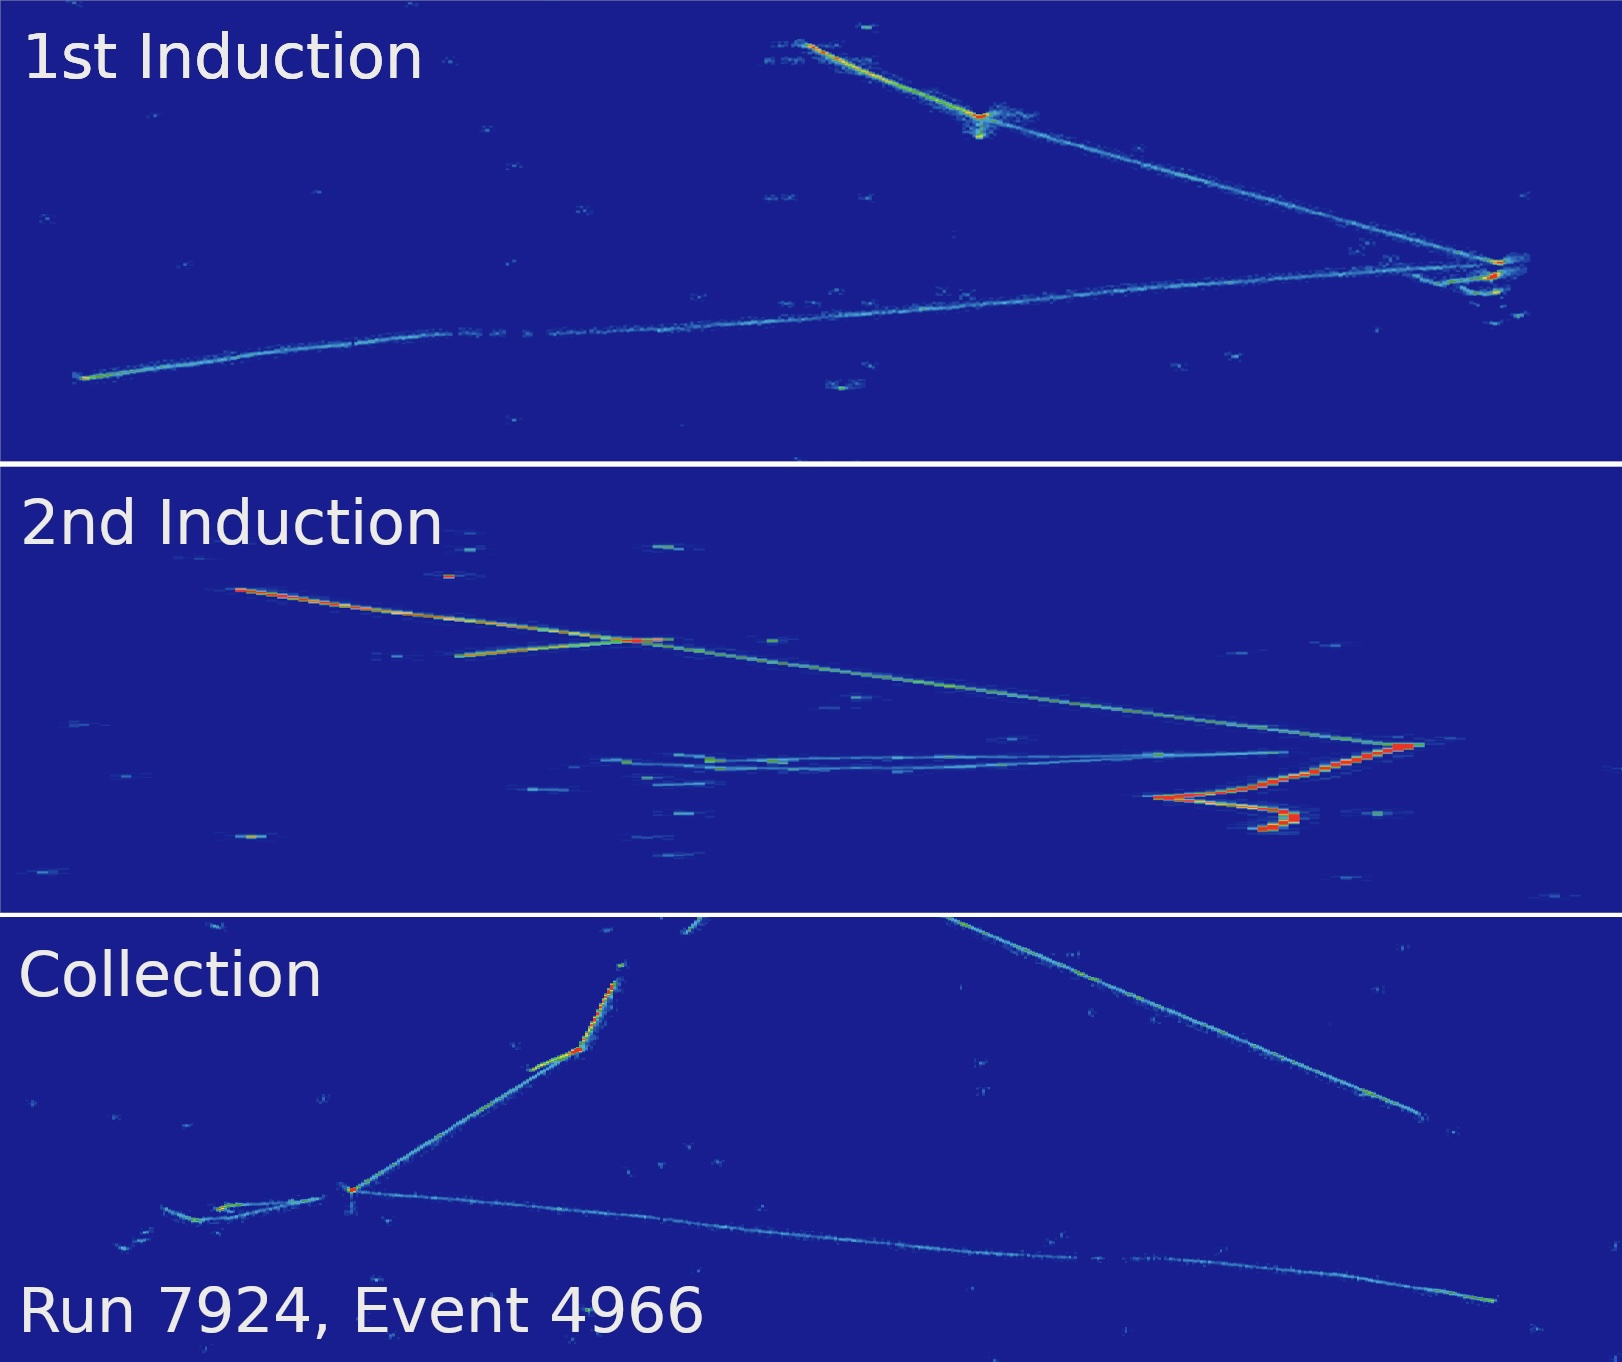
\includegraphics[width=0.45\textwidth]{figures/mlreco/mlreco_2d.jpg}
    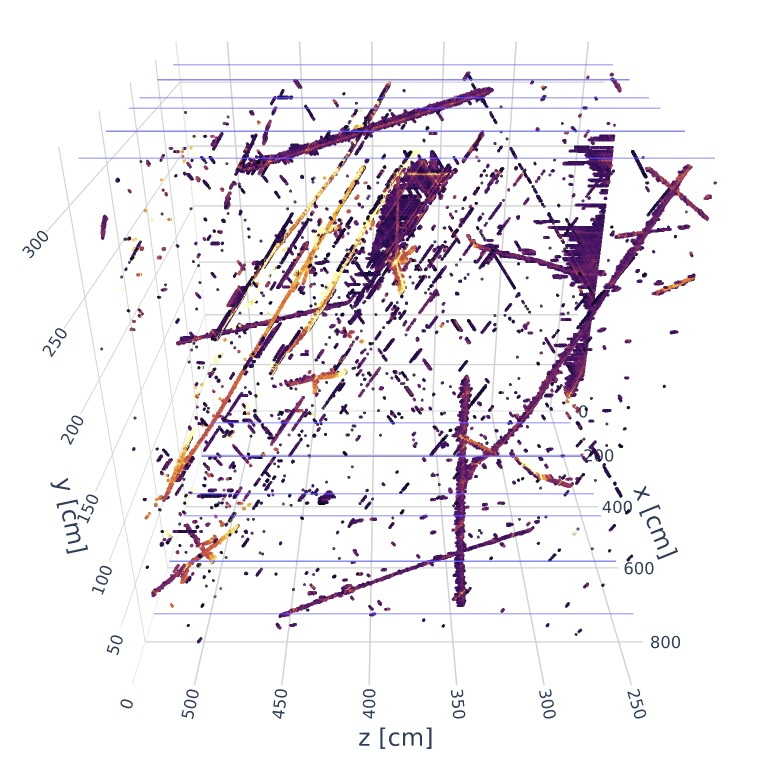
\includegraphics[width=0.45\textwidth]{figures/mlreco/mlreco_cluster3d.jpg}
    \caption{Example of a 2D event display of the same neutrino interaction in the ICARUS detector (left) and the corresponding 3D space points reconstructed by the Cluster3D algorithm (right). The image shown is a data event from Run 1.}
    \label{fig:cluster3d}
\end{figure}

\subsubsection{Point Classification}
\label{sec:point_classification}

\paragraph{Ghost point removal}
As a first step, the reconstruction is tasked with the removal of the tomographic artifacts, or ghost points, from Cluster3D (``deghosting''). The neural network used for this implements the U-ResNet architecture, which was first popularized due to its success in biomedical imaging \cite{Ronneberger2015}, to perform a binary classification of the space points, or semantic segmentation. Modifications were made to adapt U-ResNet to the sparse format of LArTPC data in contrast to regular images where each pixel contains information \cite{Domine2020b}. After deghosting, the reconstructed charge from Cluster3D is redistributed to enforce conservation of the overall charge. This is done by counting the number of times a given 2D hit is associated with a 3D space point and distributing the charge equally. The charge assigned to each space point is the average of the charge measured on each plane that contributed to the hit. An example image showing the 3D space points after the deghosting step is shown in Figure \ref{fig:deghosted}.

\begin{figure}
    \centering
    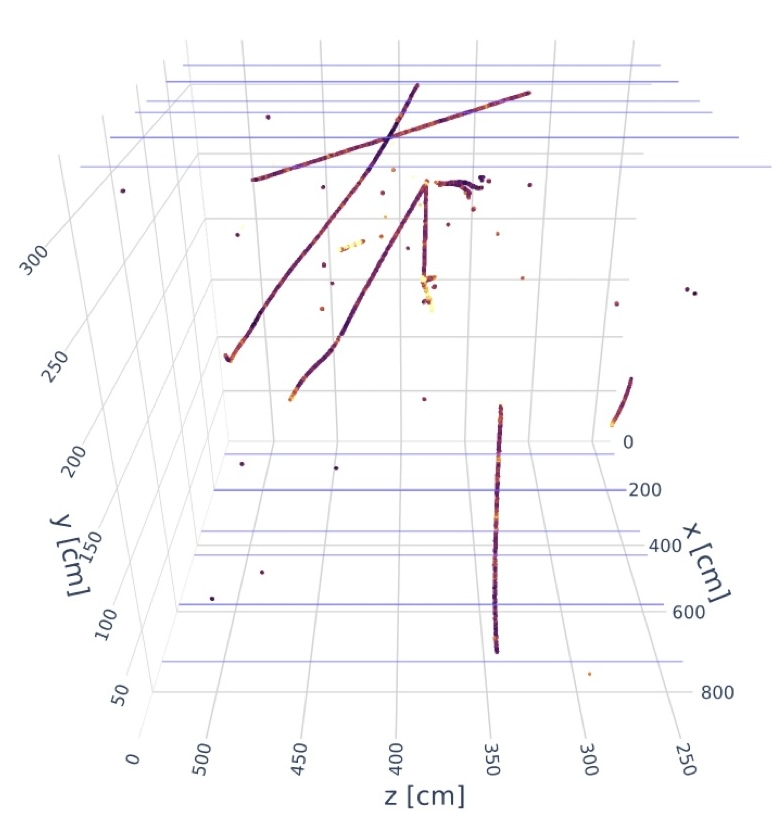
\includegraphics[width=0.6\textwidth]{figures/mlreco/mlreco_deghosted.jpg}
    \caption{Example of the 3D space points after the deghosting step. The image shown is a data event from Run 1 and the same as in Figure \ref{fig:cluster3d}.}
    \label{fig:deghosted}
\end{figure}

\paragraph{Semantic segmentation and point proposal network}
The next step in the point classification task is to classify the deghosted 3D space points into categories based on the type of parent activity that created them. The neural network used for this is a U-ResNet architecture, this time with five semantic classes of space points: Michel electron, delta ray, electromagnetic shower, track, and low-energy deposition. Each point is assigned a score for each class, and the class with the highest score is taken as the prediction. The semantic type of the space points is used in later stages of the reconstruction.

The point proposal network (PPN) is a neural network that is tasked to propose the 3D space points that are the initial and terminal points of track-like objects and the initial points of shower-like objects \cite{Domine2020a}. The PPN shares the same encoding backbone as the semantic segmentation network as shown schematically in Figure \ref{fig:mlreco_schematic}. The points of interest proposed by this network are valuable for high-level physics analyses (e.g.,\ particle start/end points and interaction vertex-finding) and are used in the clustering tasks in the later stages of the reconstruction. Figure \ref{fig:mlreco_points} shows the 3D space points colored by semantic class and the points proposed by the PPN.

\begin{figure}
    \centering
    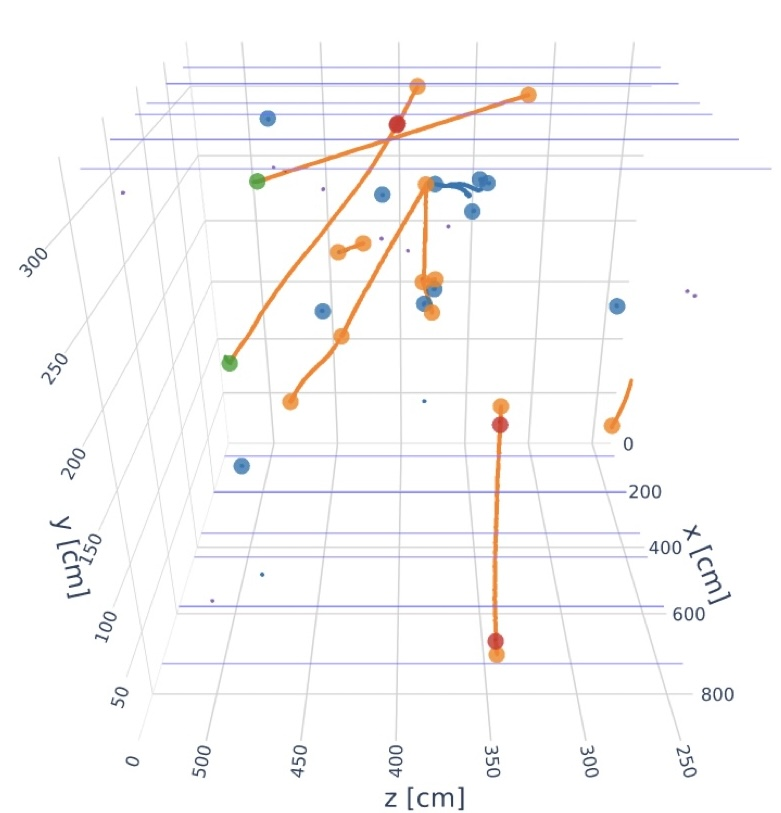
\includegraphics[width=0.45\textwidth]{figures/mlreco/mlreco_points.jpg}
    \caption{Example showing the 3D space points after the semantic segmentation and PPN stage. The space points are colored by the semantic type assigned by this stage (notably orange represents tracks, blue represents showers, green represents Michel electrons, and red represents delta rays). Also shown are the points of interest proposed by the PPN colored by the semantic class. The image shown is a data event from Run 1 and the same as in Figures \ref{fig:cluster3d} and \ref{fig:deghosted}.}
    \label{fig:mlreco_points}
\end{figure}

\paragraph{Point clustering}
The final step in the point classification task is to cluster the 3D space points in a set of points belonging to the same activity, i.e. track and shower fragments. This network, named Graph-SPICE, also uses a U-ResNet architecture and is tasked with learning an embedding of the space points in a higher-dimensional space where the points belonging to the same activity are close together. In this embedded space, the points belonging to the same semantic class are used to build a $k$-nearest neighbors graph, which connects the points that are close together. Each edge is given a score based on the feature vectors of the two points it connects and the edge is activated if the score is above a threshold. Space points are clustered into fragments by finding the connected components of the graph. The output of this stage is a set of point clusters, each representing a track or shower fragment. A paper detailing the Graph-SPICE network is in preparation.

\subsubsection{Formation of Particles and Interactions}
\label{sec:particle_interaction_reconstruction}

\paragraph{Particle instance clustering}
At this point in the reconstruction, groups of space points corresponding to particle fragments have been identified. The next step is to cluster these groups into particles. The neural network used for this task is a GNN that is tasked with a binary (on/off) edge classification, where an activated edge indicates that the two instances belong to the same particle. Two distinct GNNs are used for particle instance clustering: GrapPA-Track and GrapPA-Shower for tracks and showers, respectively. It is worth noting that these two GNNs have identical architecture and only differ in the tasks for which they have been trained. The details of the architecture of these GNNs are described in \cite{Drielsma2021}.

The node features in each GNN are mostly geometric quantities such as the particle fragment direction vector and the most-likely PPN point. Edge features are also geometry-based and include the distance between the two fragments. The initial state of the graph has activated edges for all node pairs up to a maximal distance. This limitation is motivated by both the computational cost associated with fully connecting an image in a detector as large as ICARUS and by physics concerns: beyond a certain length scale there cannot be legitimate connections. The result of these two GNNs is a set of complete particles of both the track and shower categories. Small gaps in tracks, for example due to track-breaking at the cathode, are expected to be resolved in this stage. The shower-clustering step also identifies the primary shower fragment that is used to identify the shower start point, a critical feature for the interaction-clustering step.

\paragraph{Interaction clustering}
The final stage of the event reconstruction is to cluster the particles into interactions, defined as a group of particles originating from the same vertex. Particles that are directly connected to the primary vertex are considered primary particles, meaning they are immediate products of the interaction, whereas other particles are labeled as secondaries. The clustering of particles into interactions is easily cast as an edge-classification task, where an activated edge indicates two particles belong to the same interaction. In addition to the interaction clustering, the network is also tasked with predicting for each node the particle type (photon, electron, muon, pion, or proton) and the primary/secondary label. The neural network used for this task is a GNN and is described extensively in \cite{Drielsma2021}. The architecture of this GNN differs from GrapPA-Track and GrapPA-Shower only in that it has more hidden features, which are useful for the extra tasks of particle identification (PID) and primary ID classification. The output of this stage is a full list of interactions in the event, each with a list of primary and secondary particles and their types.

\subsection{Post-Processing}
\label{sec:post_processing}

After the full chain of neural networks has been applied to the event, the output is a list of interactions with their associated particles. Each particle has been designated as a primary or secondary particle and has had a particle type assigned. In addition to this high-level set of information, a full physics analysis requires further information to be extracted from the event. This includes kinematic information such as the momentum and energy of the particles, as well as other geometric information such as the interaction vertex location. Association of interactions with the corresponding optical flash provides precise timing that can be leveraged in analyses. This information is extracted using traditional reconstruction algorithms that are well-established in the field of neutrino physics. 

\subsubsection{Kinematic Reconstruction}
\label{sec:kinematic_reconstruction}

The kinematic reconstruction of the particles in the event is performed using traditional reconstruction algorithms. Of relevance for the analysis presented here are the following reconstructed quantities:

\begin{itemize}
    \item \textbf{Particle direction reconstruction}: The direction of the particle at the start (tracks and showers) and end (tracks only) points is reconstructed using a principal component analysis (PCA) of the space points in the local neighborhood of the point. When combined with the kinetic energy of the particle, the momentum (direction and magnitude) can be reconstructed.
    \item \textbf{Calorimetric energy reconstruction}: The energy of the particle is reconstructed using the total charge deposited by the particle in the detector. The charge is converted to energy using an effective formula that accounts for the average amount of electron-ion recombination, the TPC electronics gain, the work function of liquid argon, the attenuation due to electron lifetime, and a scale factor that accounts for the missed shower fragments that have fallen below the detection threshold. This is most useful for showers, for which other methods of energy reconstruction are not available.
    \item \textbf{Track length reconstruction}: The length of the track is reconstructed by segmenting the track and summing the length of each segment along their respective principal axes. 
    \item \textbf{Range-based energy reconstruction}: The energy of the track is estimated using the well-known relationship between the kinetic energy of a particle and its range in a material according to the Bethe-Bloch formula. This relation is known as the Continuous Slowing Down Approximation (CSDA) and it is used to estimate the energy of the particle. This method assumes that the particle ranges out in the argon without nuclear interactions and that the track is fully contained in the detector.
    \item \textbf{Vertex reconstruction}: The interaction vertex is reconstructed as the point joining the start points of the primary particles in the interaction.
    \item \textbf{Fiducial volume}: The interaction vertex is used to determine if the interaction occurred within the fiducial volume of the detector. This is defined as the region \qty[mode=text]{25}{cm} from the edges of the detector in the $x$ and $y$ directions, \qty[mode=text]{30}{cm} from the upstream edge in the $z$ direction, and \qty[mode=text]{50}{cm} from the downstream edge in the $z$ direction. These numbers were assumed in the SBN proposal \cite{Acciarri2015} and are chosen to avoid reconstruction inefficiencies near the edges of the detector (e.g.\ exiting particles that are not seen).
    \item \textbf{Containment}: The containment of the particles in the detector is determined by requiring that all the space points of the particle are at least \qty[mode=text]{5}{cm} from the edges of the detector. At the interaction level, the interaction is considered contained if all of the particles that comprise it are contained. The containment cut also applies the constraint that the space points must be in the same TPC that created them; out-of-time tracks may be reconstructed partially in the wrong TPC and therefore be removed by this cut. The value of \qty[mode=text]{5}{cm} was chosen based on the expected magnitude of space charge effects in the detector, which tends to displace space points away from the detector boundaries.
\end{itemize}

\subsubsection{Optical Flash Association}
\label{sec:optical_flash_association}

The optical flash is a prompt signal in the PMTs associated with the scintillation light produced by the neutrino interaction in the detector. As part of the standard reconstruction chain, the optical flash is formed from optical hits, which themselves are reconstructed from the PMT waveforms. This flash object can be thought of as a set of optical hits each with a well-defined position, time, and photoelectron count. The job of the flash association algorithm is to leverage these characteristics and match them to the interactions in the event that are imaged by the TPC through detection of ionization charge signals.

The tool used for flash association is a package originally developed for MicroBooNE called OpT0Finder. OpT0Finder employs a likelihood-based approach to match the optical flash to charge activity associated with an interaction in the event. For each interaction, as defined by the upstream ML reconstruction, the algorithm calculates an allowed range of $x$ offsets that are allowed by the geometry. This reflects our inability to know beforehand the exact time of the interaction. For each of these allowable positions\footnote{This is not actually a brute-force algorithm, but rather an optimization algorithm that profiles across the drift direction.}, the algorithm calculates a hypothesis flash based on the expected light yield of the interaction, the distribution of the ionization charge in the interaction, and the position of the PMTs in the detector. The hypothesis flash and the observed flash each have a likelihood computed using a joint probability distribution of the photoelectron count in each PMT given the $x$ position of the flash. Maximizing the likelihood between the two allows the assignment of a score to each potential interaction-flash pair. 

A matching algorithm then selects the best pairings based on the scores while simultaneously skipping pairs with an already matched flash or interaction. The result of this association process is the assignment of a time stamp to each interaction which was successfully matched to a flash. This time stamp can be used to precisely tag an interaction as being in-time or out-of-time with respect to the beam spill, and therefore can be leveraged as a tool for cosmic rejection.